\chapter{Einleitung}
\label{sec: Einleitung}

\section{Aufgabenstellung}
    % Allgemeine Aufgabenstellung
    %----------------------------
    Im Zuge dieser Laborübung soll ein Modellflugzeug schwingungstechnisch
    untersucht werden. Dabei gilt es, 4 verschiedene Aufgabenstellungen
    abzuhandeln. Um die Leserlichkeit zu erleichtern, werden die einzelnen
    Aufgabenstellung in eigenen Unterkapiteln jeweils vollständig abgearbeitet.
%================================================================================

\section{Vorbereitung}
    % Aufbereitung des Modellflugzeugs
    %---------------------------------
    Da für die folgenden Messungen oftmals lineare Zusammenhänge angenommen
    werden, sollen im vermessenen System möglichst keine Nichtlinearitäten
    vorkommen. Deshalb werden lose Flugzeugteile (z.B. lose hängende Ketten,
    wackelnde Finnen, ...) mit Klebeband fixiert.
    Konkret wurden beim verwendeten Modellflugzeug folgende Teile befestigt:

    % Aufzählung der befestigen Teile
    %--------------------------------
    \begin{itemize}
        \item eine lose hängende Kette vorne beim Motor
        \item die Mittelfinne am Heck
        \item das Fahrwerk am Heck
    \end{itemize}
    %----------------------------------------------------------------------------

    % Bilder des aufbereiteten Flugzeugs
    %-----------------------------------
    \noindent
    Das für die Versuche aufbereitete Modellflugzeug kann den Abbildungen
    \ref{fig: Modellflugzeug_vorbereitet} bis \ref{fig: Kette_fixiert} entnommen
    werden. Die Stellen, an denen lose Bauteile fixiert wurden, sind dabei mit
    roten Ellipsen gekennzeichnet.

    % Bild - Flugzeug aufbereitet
    %----------------------------
    \begin{figure}[H]
        \centering
        \includegraphics[width=0.45\textwidth]{Flieger_aufbereitet.png}
        \caption{Modellflugzeug ohne Nichtlinearitäten}
        \label{fig: Modellflugzeug_vorbereitet}
    \end{figure}

    % Bild - hinteres Fahrwerk
    %-------------------------
    \begin{figure}[H]
        \centering
        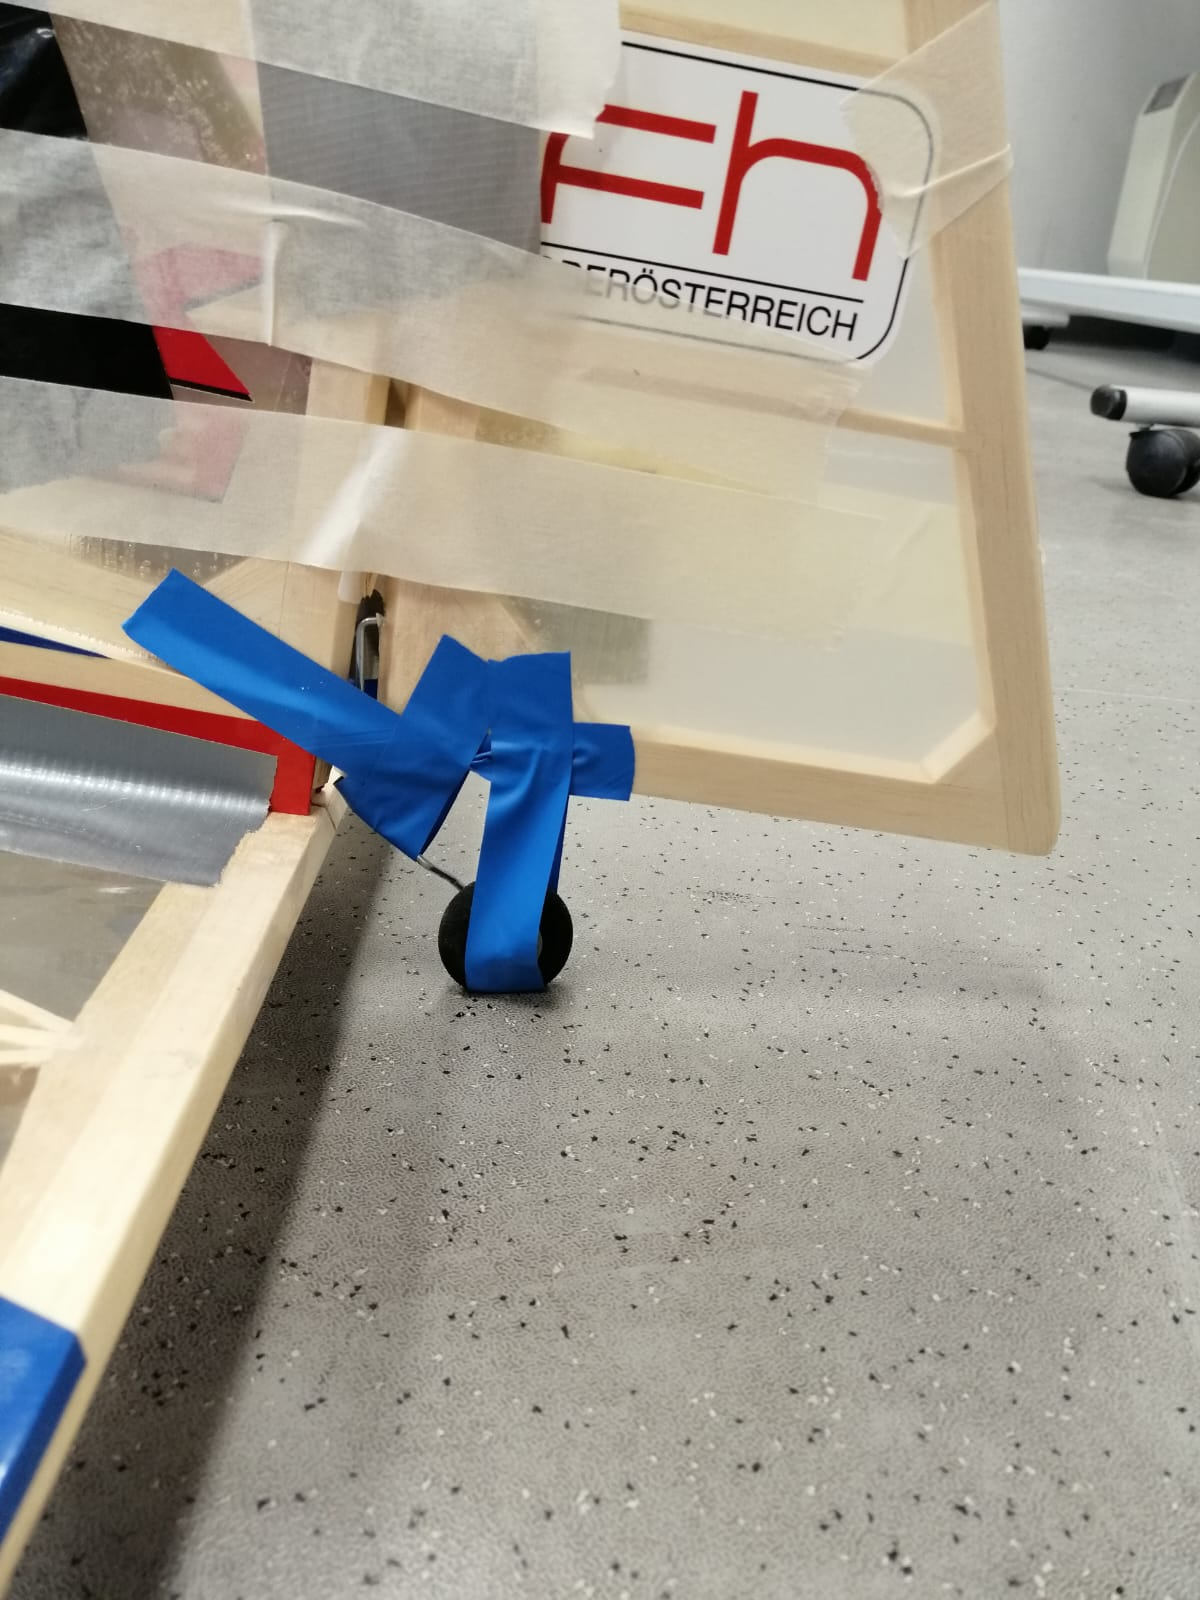
\includegraphics[width=0.5\textwidth]{fixiertes_Hinterrad.png}
        \caption{Fixierung des hinteren Fahrwerks}
        \label{fig: Hinterrad_fixiert}
    \end{figure}

    % Bild - Kettenbefestigung
    %-------------------------
    \begin{figure}[H]
        \centering
        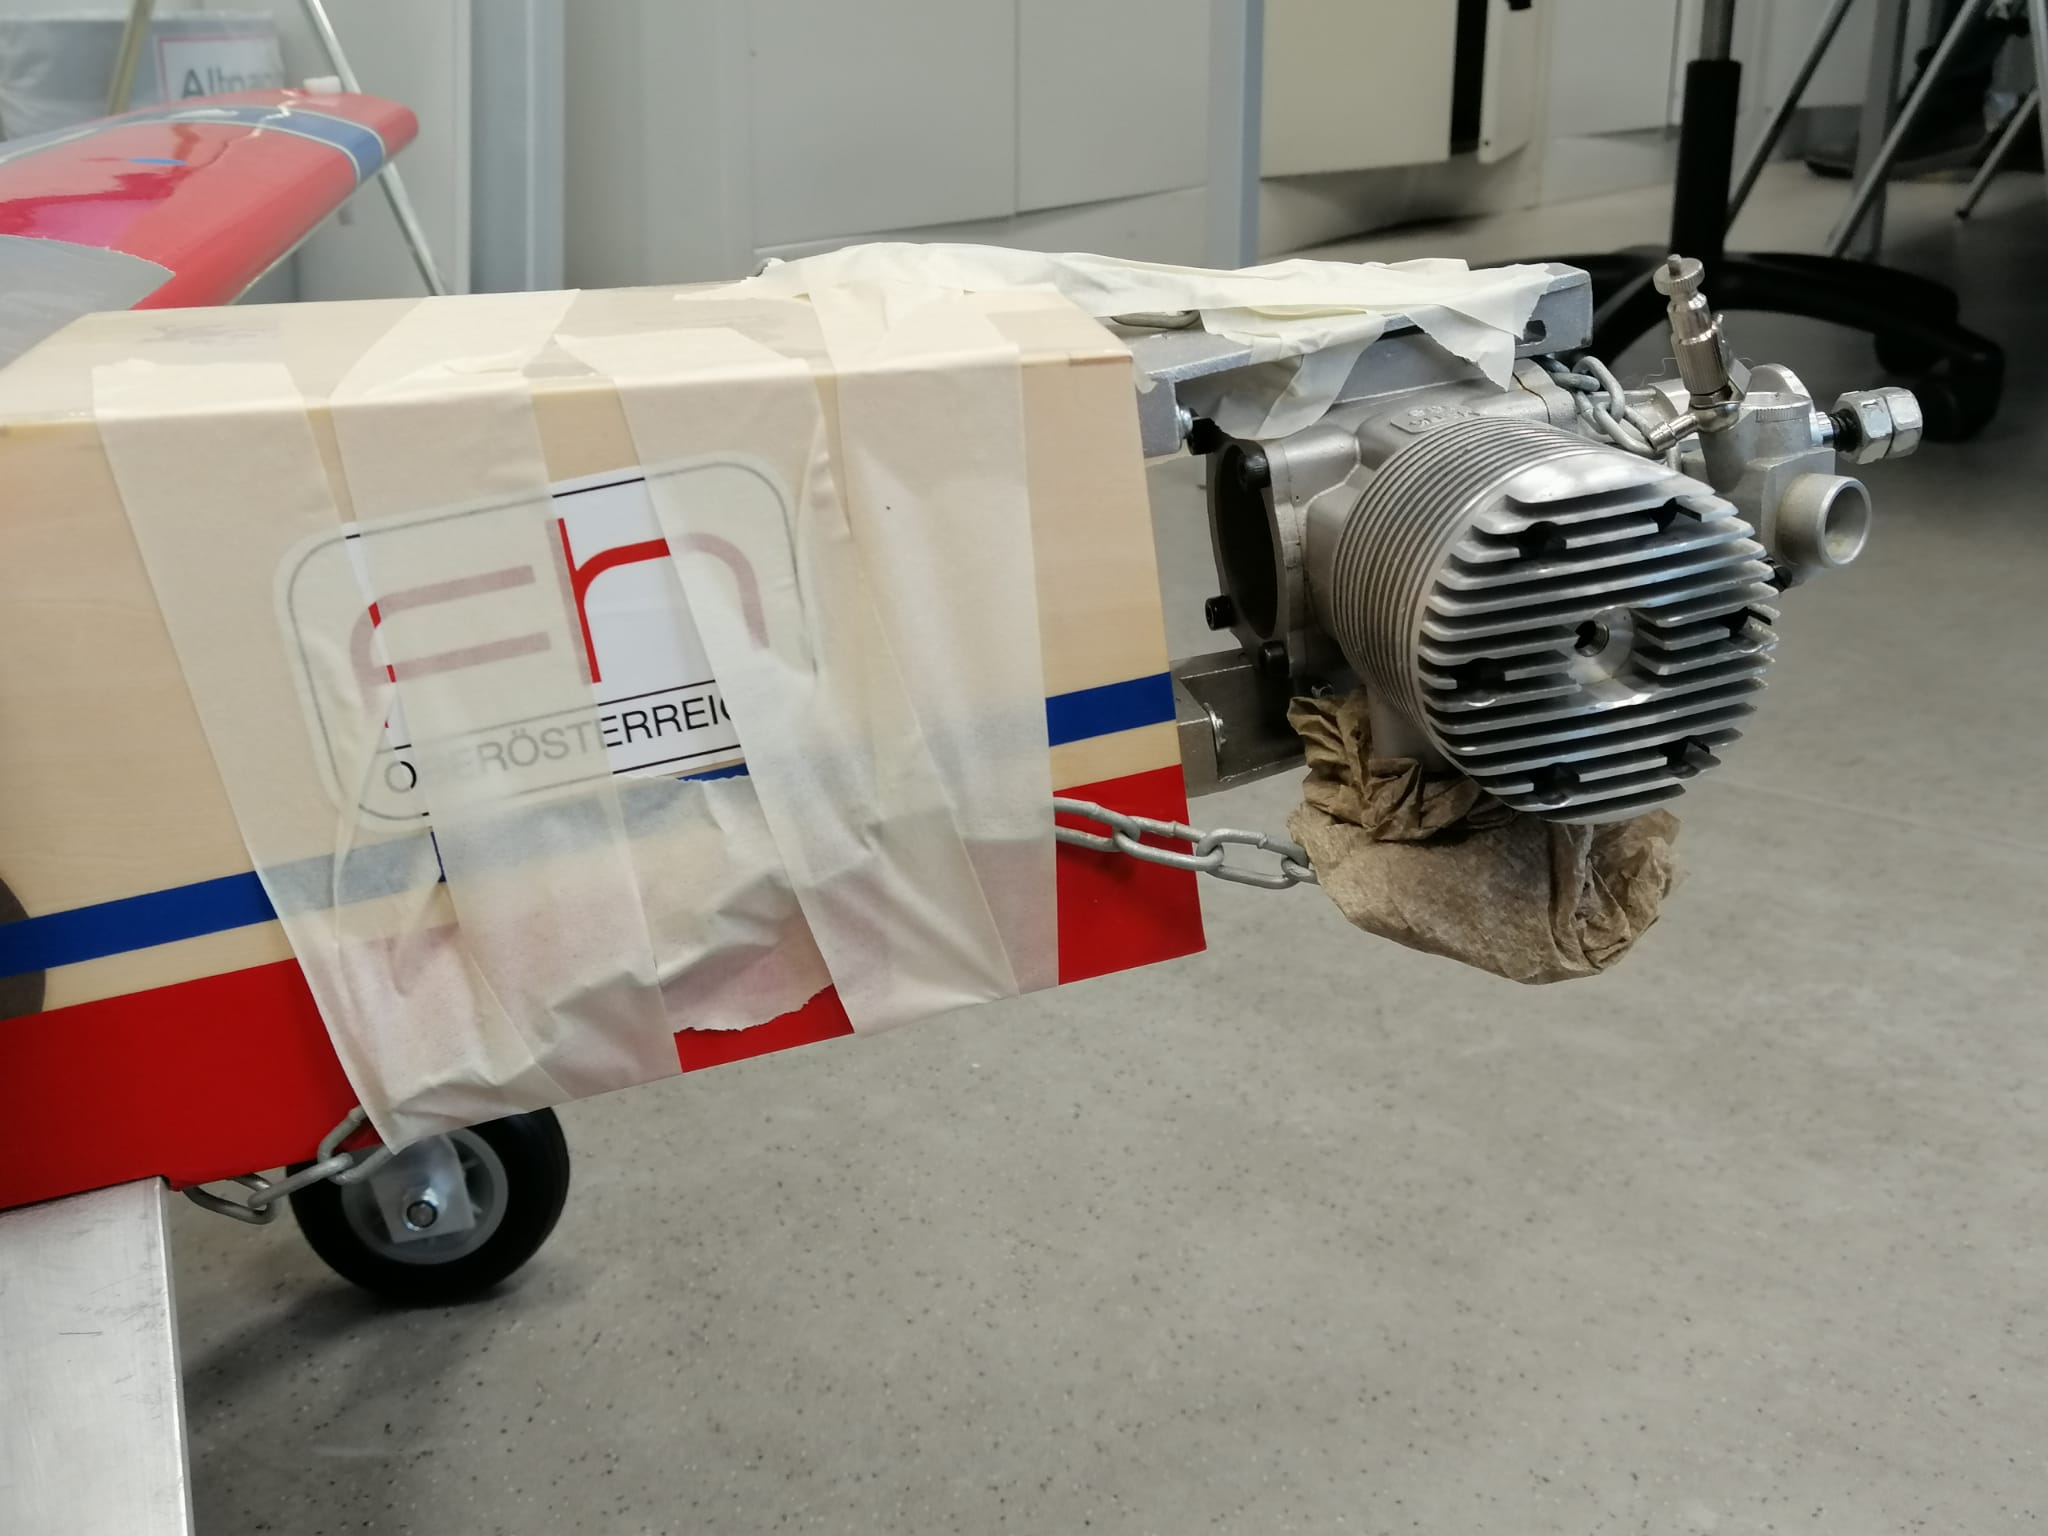
\includegraphics[width=0.5\textwidth]{Kette_fixiert.png}
        \caption{Fixierung der Kette}
        \label{fig: Kette_fixiert}
    \end{figure}
